\documentclass{article}
\usepackage[utf8]{inputenc}
\usepackage{graphicx}
\usepackage{amsmath}
\usepackage[
backend=biber,
style=alphabetic,
sorting=ynt
]{biblatex}
\addbibresource{references.bib} 
\graphicspath{ {images/} }

%opening
\title{YOUR TITLE}
\author{YOUR FULL NAME \thanks{Green Global Information Technology JSC}}
\date{\today}

\begin{document}

\maketitle

% The introduction
\begin{abstract}
Machine learning is a set of powerful mathematical tools that enable us, to represent, interpret, and control the complex world around us.
However, even just the word mathematics makes some people feel uneasy and unwelcome to explore the topic.
The purpose of this session is to take you on a tour through the basic maths underlying these methods, focusing in particular on building your intuition rather than worrying too much about the details.
Thanks to the amazing machine learning community, it's actually possible to apply many powerful machine learning methods without understanding very much about the underpinning mathematics, by using open source libraries.
This is great, but problems can arise and without some sense of the language and meaning of the relevant maths, you can struggle to work out what's gone wrong or how to fix it.
The ideal outcome of this session is that it will give you the confidence and motivation to immediately dive into one of the hundreds of boolean applied machine learning courses already available online, and not be intimidated by the matrix notation or the calculus.
\end{abstract}

% The first section's topic
% Every section is a main idea for what you have learnt
\section{Introduction to Linear Algebra and to Mathematics for Machine Learning}

In this first module we look at how linear algebra is relevant to machine learning and data science. Then we'll wind up the module with an initial introduction to vectors. Throughout, we're focusing on developing your mathematical intuition, not of crunching through algebra or doing long pen-and-paper examples. For many of these operations, there are callable functions in Python that can do the adding up - the point is to appreciate what they do and how they work so that, when things go wrong or there are special cases, you can understand why and what to do.

\subsection{Learning Objectives}

\begin{itemize}
	\item Recall how machine learning and vectors and matrices are related
	\item Interpret how changes in the model parameters affect the quality of the fit to the training data
	\item Recognize that variations in the model parameters are vectors on the response surface - that vectors are a generic concept not limited to a physical real space
	\item Use substitution / elimination to solve a fairly easy linear algebra problem
	\item Understand how to add vectors and multiply by a scalar number
\end{itemize}

\subsection{Subsection's name}

\subsection{The relationship between machine learning, linear algebra, and vectors and matrices}

\subsubsection{Motivations for linear algebra}

We're going to look a bit more at the types of problems we might want to solve, and expose what Linear Algebra is and how it might help us to solve them.
The first problem I might think of is one of price discovery.

\begin{equation} \label{eq1}
\begin{split}
2a + 3b & = 8 \\
10a + 1b & = 13
\end{split}
\end{equation}

Say I go shopping on two occasions, and I buy apples and bananas, and the first time I buy two apples and three bananas and they cost eight Euros.
And the second time I buy say, ten apples and one banana, and the cost is 13 Euros.
And the \textbf{As} and the \textbf{Bs} here,
are the price of a \textbf{single apple} and a \textbf{single banana}.
And what I'm going to have to do is \textbf{solve} these what we call \textbf{\textit{simultaneous equations}} in order to discover the price of individual apples and bananas.

Now in the general case of lots of different types of items and lots of shopping trips, then finding out the prices might be quite hard. It might be quite \textit{difficult} to \textit{solve} all these equations \textit{by hand}. So, we might want a \textit{computer algorithm} to do it for us, in the general case. Now, this is an example of a \textit{Linear Algebra} problem.

\begin{equation} \label{eq2}
	\begin{bmatrix}
	2 & 3 \\
	10 & 1
	\end{bmatrix}
	\cdot
	\begin{bmatrix}
	a \\
	b
	\end{bmatrix}
	=
	\begin{bmatrix}
	8 \\
	13
	\end{bmatrix}
\end{equation}

I have some \textbf{constant} \textit{linear coefficients} here, these numbers \textit{2, 10, 3, 1}, that relate the \textbf{input} variables A and B, to the \textbf{output} 8 and 13, that is if I think about a vector [a,b], that describes the prices of apples and bananas.

Looking at these different types of mathematical objects, and understanding what they are and how to work with them, these \textit{vectors} and \textit{matrices}. In fact, with neural networks and machine learning, we want the computer in effect \textbf{\textit{not only}} to fit the equation, \textbf{\textit{but also}} to figure out what equation to use. That's a highly inexact description really of what's going on, but it gives the right sort of flavor.

\subsubsection{Getting a handle on vectors}

\subsubsection{Exploring parameter space}

\subsubsection{Solving some simultaneous equations}

\subsection{Operations with vectors}

\section{Second Section}

% The Conclusion
\section{Recap}

In this session of our course on Linear Algebra, I first looked at the problem of data, that our world has so much of it.
Then, if we could figure out how to analyze and use it, we could really solve problems in the world.
Moreover, we've looked at where these courses fit in terms of helping us access the world of machine learning and data science.
Then we've moved on to look at some example problems, the problem of solving some simultaneous equations. For example, to discover the price of things in the apples and bananas problem, or the problem of fitting a model equation with some fitting parameters we want, to optimize against some data.
We've then said that both of these problems are going to involve vectors and possibly some calculus. Therefore, we've started off our journey with vectors and with defining vector addition and scalar multiplication.

% Your plan in the next week.
In the next week, I'll do research how Machine Learning can be used to convert Fahrenheit to Celsius.

\begin{figure}[h]
\centering
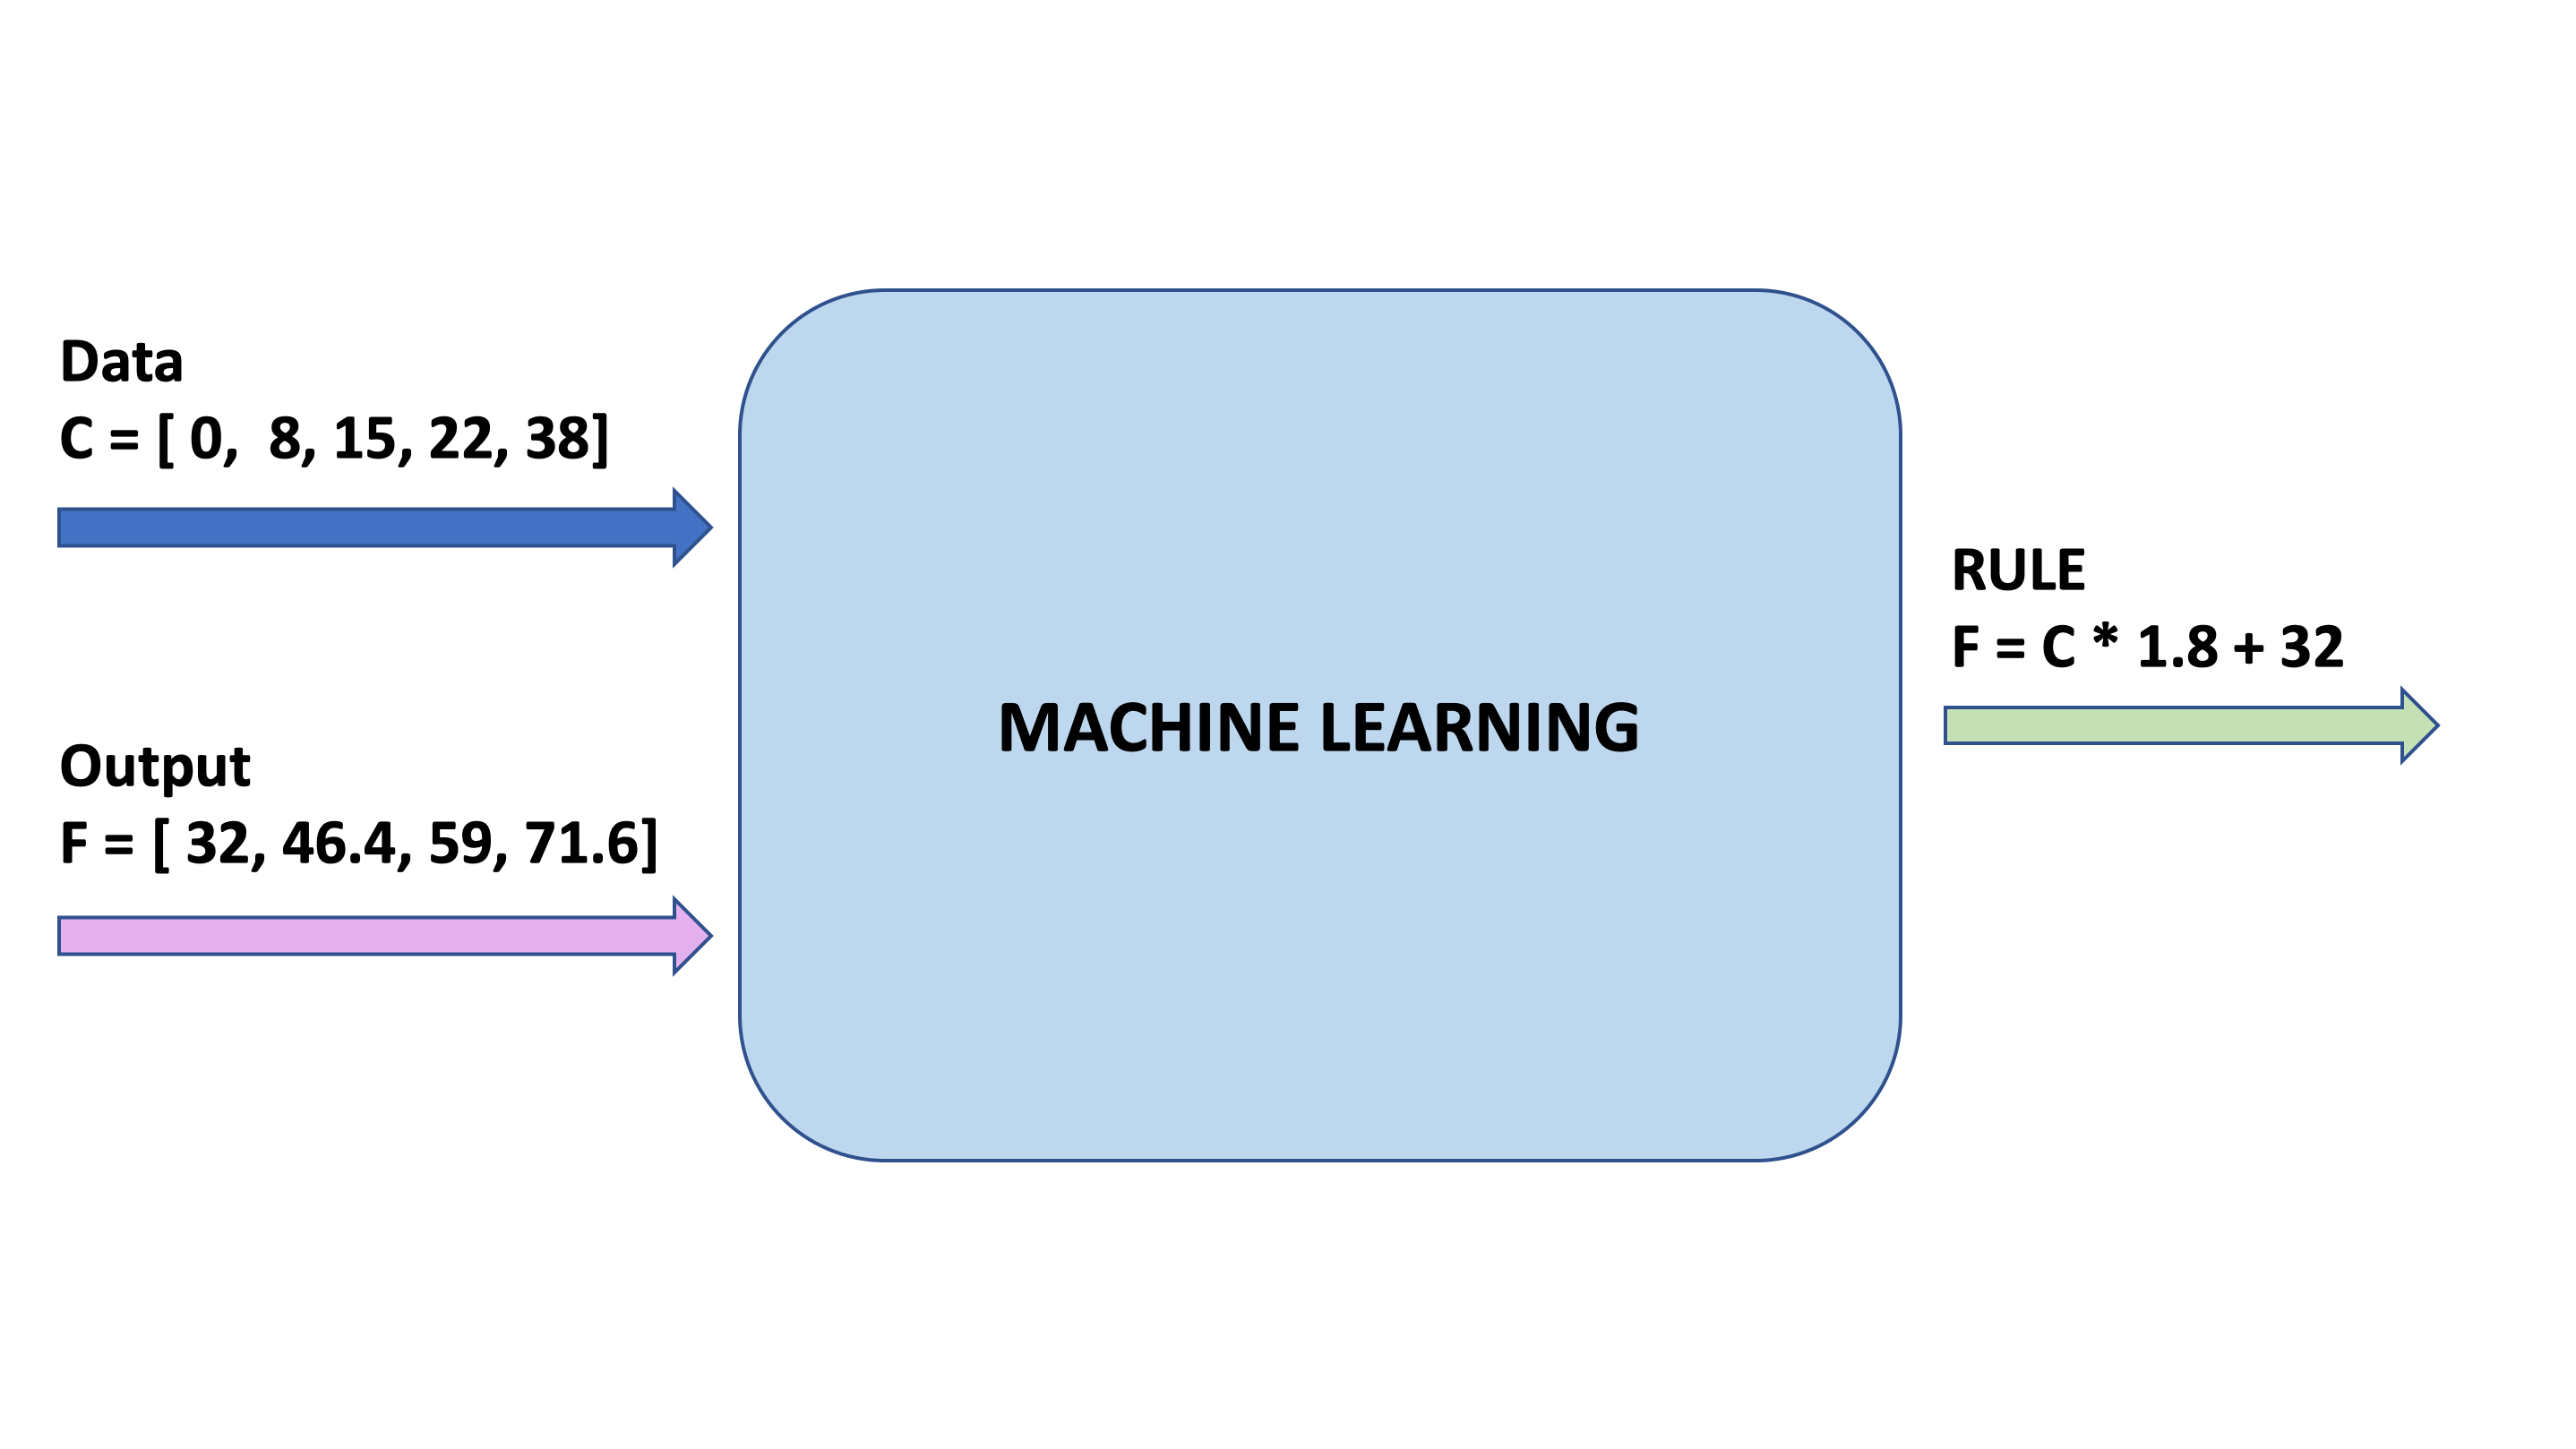
\includegraphics[width=8cm]{tensorflow-l2f1}
\caption{Converting Fahrenheit to Celsius}
\label{fig:F2C}
\end{figure}

The figure \ref{fig:F2C} illustrates how Machine Learning can be used to convert Fahrenheit to Celsius.

\nocite{*}

\printbibliography

\end{document}